% This file was created by tikzplotlib v0.9.8.
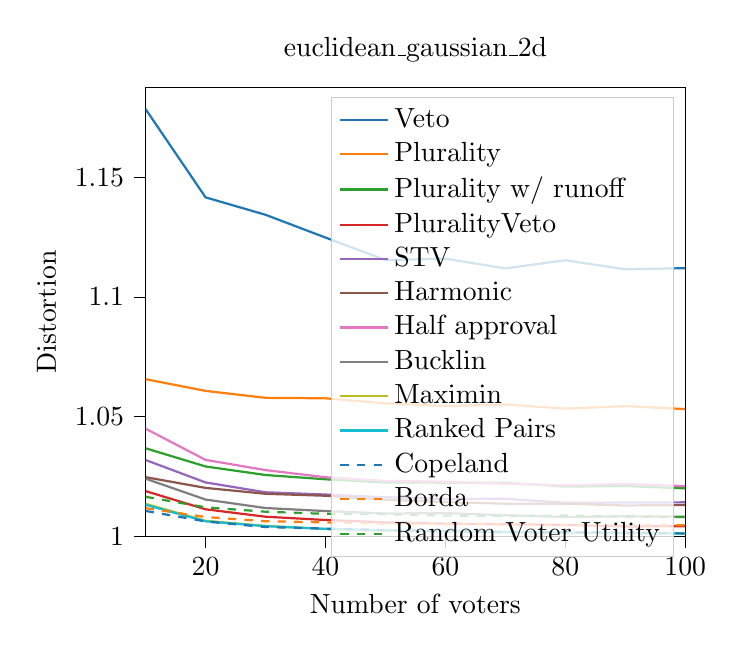
\begin{tikzpicture}

\definecolor{color0}{rgb}{0.12156862745098,0.466666666666667,0.705882352941177}
\definecolor{color1}{rgb}{1,0.498039215686275,0.0549019607843137}
\definecolor{color2}{rgb}{0.172549019607843,0.627450980392157,0.172549019607843}
\definecolor{color3}{rgb}{0.83921568627451,0.152941176470588,0.156862745098039}
\definecolor{color4}{rgb}{0.580392156862745,0.403921568627451,0.741176470588235}
\definecolor{color5}{rgb}{0.549019607843137,0.337254901960784,0.294117647058824}
\definecolor{color6}{rgb}{0.890196078431372,0.466666666666667,0.76078431372549}
\definecolor{color7}{rgb}{0.737254901960784,0.741176470588235,0.133333333333333}
\definecolor{color8}{rgb}{0.0901960784313725,0.745098039215686,0.811764705882353}

\begin{axis}[
legend cell align={left},
legend style={fill opacity=0.8, draw opacity=1, text opacity=1, draw=white!80!black},
tick align=outside,
tick pos=left,
title={euclidean\_gaussian\_2d},
x grid style={white!69.0196078431373!black},
xlabel={Number of voters},
xmin=10, xmax=100,
xtick style={color=black},
y grid style={white!69.0196078431373!black},
ylabel={Distortion},
ymin=1, ymax=1.1874717696172,
ytick style={color=black}
]
\addplot [thick, color0]
table {%
10 1.17859668746434
20 1.14168822925457
30 1.13440309810232
40 1.1248785095104
50 1.11546900426379
60 1.11604418474111
70 1.11197698949928
80 1.11539852197379
90 1.11159743538065
100 1.11207829930305
};
\addlegendentry{Veto}
\addplot [thick, color1]
table {%
10 1.06565533384075
20 1.06075907196425
30 1.05785595369635
40 1.05766885437416
50 1.05556480677277
60 1.05441676140157
70 1.05509707628674
80 1.0533233320174
90 1.05441512858796
100 1.05314664657491
};
\addlegendentry{Plurality}
\addplot [thick, color2]
table {%
10 1.03676130909163
20 1.0291620841293
30 1.02558483733042
40 1.02379897206898
50 1.02244998754484
60 1.02238017797179
70 1.02232866244329
80 1.02075480262214
90 1.02097155930585
100 1.02000240438466
};
\addlegendentry{Plurality w/ runoff}
\addplot [thick, color3]
table {%
10 1.01885922964912
20 1.01124778449038
30 1.00814468819877
40 1.00676974959466
50 1.0057691475562
60 1.0052268885317
70 1.004993739777
80 1.00470231479086
90 1.00407162698384
100 1.00417561981997
};
\addlegendentry{PluralityVeto}
\addplot [thick, color4]
table {%
10 1.03185656232961
20 1.02247957726457
30 1.01835638407585
40 1.01742707700564
50 1.01629375810831
60 1.01555967705263
70 1.01565478891384
80 1.01393885250775
90 1.0140759635806
100 1.01415457283434
};
\addlegendentry{STV}
\addplot [thick, color5]
table {%
10 1.02468234864817
20 1.0201951286168
30 1.01773172401148
40 1.0169135478224
50 1.01524571408369
60 1.01428724924928
70 1.01358615675696
80 1.01356524750363
90 1.01284953110079
100 1.01302125868214
};
\addlegendentry{Harmonic}
\addplot [thick, color6]
table {%
10 1.04495068738702
20 1.0319060840942
30 1.02764051287934
40 1.02464618123342
50 1.02313990329202
60 1.02277257667666
70 1.02190005246565
80 1.02131805167826
90 1.02184532714433
100 1.02092427565619
};
\addlegendentry{Half approval}
\addplot [thick, white!49.8039215686275!black]
table {%
10 1.02403455235844
20 1.01532918333756
30 1.01177179509093
40 1.01050745893298
50 1.00950508846443
60 1.00963756410517
70 1.00876232912534
80 1.0080318653799
90 1.0083259983274
100 1.00813762256002
};
\addlegendentry{Bucklin}
\addplot [thick, color7]
table {%
10 1.01353686264864
20 1.00644172413292
30 1.00430505257558
40 1.00300101119482
50 1.00213437522728
60 1.00202741607367
70 1.00166191506182
80 1.0015034986009
90 1.00145702748747
100 1.00112227334724
};
\addlegendentry{Maximin}
\addplot [thick, color8]
table {%
10 1.01313280233302
20 1.00621833708636
30 1.00418606719397
40 1.00307951975713
50 1.00248547248846
60 1.00207432487104
70 1.00173785351493
80 1.00150446342992
90 1.00133576090589
100 1.00109504440715
};
\addlegendentry{Ranked Pairs}
\addplot [thick, color0, dashed]
table {%
10 1.01056591028462
20 1.00617294794544
30 1.00382008258589
40 1.0031819042856
50 1.00258052862264
60 1.00208392086749
70 1.00181325020153
80 1.00161491964531
90 1.00145235730775
100 1.00115211080218
};
\addlegendentry{Copeland}
\addplot [thick, color1, dashed]
table {%
10 1.01170635243131
20 1.00802057031156
30 1.00624791077111
40 1.00578171697542
50 1.00521778805456
60 1.00501220761806
70 1.00491519303267
80 1.00468268535718
90 1.00454824546892
100 1.00459198961809
};
\addlegendentry{Borda}
\addplot [thick, color2, dashed]
table {%
10 1.01647369017238
20 1.01207235833286
30 1.01023987583749
40 1.00934539496311
50 1.00921477908704
60 1.00864494229119
70 1.00839490899459
80 1.00865688585786
90 1.00813845007054
100 1.00799514924622
};
\addlegendentry{Random Voter Utility}
\end{axis}

\end{tikzpicture}
